\documentclass[11pt]{exam}

\usepackage{amsmath}
\usepackage{graphicx}
\usepackage{geometry}
\usepackage{etoolbox}
\BeforeBeginEnvironment{choices}{\par\nopagebreak\minipage{\linewidth}}
\AfterEndEnvironment{choices}{\endminipage}
\geometry{
a4paper,
total={185mm,257mm},
left=10mm,
top=25mm,
bottom=10mm
}

\begin{document}
\setlength{\voffset}{-0.5in}
\setlength{\headsep}{5pt}

\fbox{\fbox{\parbox{8cm}{\centering
\vspace{2mm}
Testat - Versuch J - Ultraschall - 2
\vspace{2mm}
}}}
\hspace{2mm}
\makebox[0.25\textwidth]{Name:\enspace\hrulefill} \hspace{5mm}
\makebox[0.2\textwidth]{Datum:\enspace\hrulefill}
\vspace{4mm}

\begin{questions}

\question Wie groß ist die Wellenlänge des in der Graphik dargestellten Signals (in Luft)? 

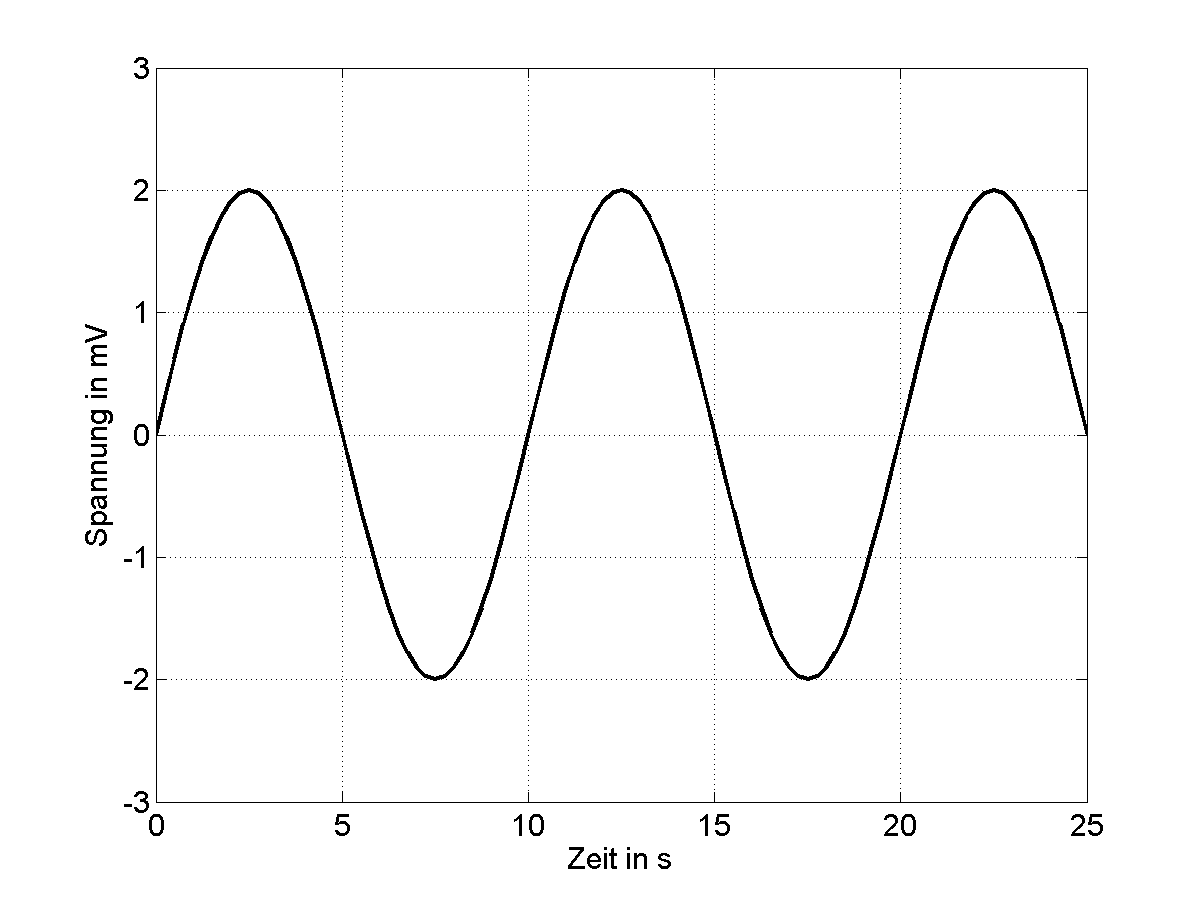
\includegraphics[width=0.5\textwidth]{../../../questions/J/images/SchallSinus1.png}

\begin{choices}
	\choice 3430 m (correct)
	\choice 25 s
	\choice 0,1 Hz
	\choice 6,86 m
	\choice 10 s
\end{choices}

\vspace{3mm}\question Mit welcher Gleichung lässt sich der zurückgelegte Weg \( s \) eines Schallsignals beschreiben?( \( t \) Laufzeit des Signals, \( c \) Schallgeschwindigkeit )

\begin{choices}
	\choice \( s= \frac{t}{c} \)
	\choice \( s=c^2 \cdot t \)
	\choice \( s=c \cdot t \) (correct)
	\choice \( s = c \cdot t^2 \)
	\choice \( s= \frac{c}{t} \)
\end{choices}

\vspace{3mm}\question Mit einem Echolot soll eine Position eines Gegenstandes in einem Medium mit einer Schallgeschwindigkeit von 100 m/s überprüft werden. Dazu wird durch eine Sonde eine Schallwelle ausgestrahlt, die an dem Gegenstand reflektiert wird und daraufhin wieder an der Sonde eintrifft. Wie lange müsste es bei einer Entfernung zwischen Gegenstand und Sonde von 25~m dauern, bis die Schallwelle nach ihrer Aussendung wieder an der Sonde eintrifft?

\begin{choices}
	\choice etwa 2 s
	\choice etwa 4 s
	\choice etwa 1 s
	\choice etwa 0,5 s (correct)
	\choice etwa 0,25 s
\end{choices}

\vspace{3mm}\question Bei welcher Frequenz \( f \) befindet sich bei einem gesunden menschlichen Durchschnittsohr die untere Hörschwelle?

\begin{choices}
	\choice 16 kHz
	\choice 20 Hz (correct)
	\choice 2000 Hz
	\choice 20 kHz
	\choice 16 MHz
\end{choices}

\vspace{3mm}\question Welche Aussagen zur Ultraschalldiagnostik sind zutreffend?	* Ultraschallgeräte funktionieren nach dem Prinzip der Laufzeitbestimmung  von Ultraschallpulsen.	* Trifft ein Ultraschallpuls auf eine Grenzfläche zwischen zwei Medien, so wird der Schall daran immer vollständig reflektiert. So entsteht ein Echo, das für die Laufzeitbestimmung genutzt werden kann.	* In einem Ultraschallgerät sind meistens zwei verschiedene Geräte, ein Ultraschall-Sender und ein Ultraschall-Empfänger, eingebaut.	* Die Reflexion von Ultraschallwellen an Gewebegrenzflächen kann mit dem aus der Optik bekannten Reflexionsgesetz beschrieben werden.

\begin{choices}
	\choice Nur 2 ist falsch.
	\choice Nur 4 ist falsch.
	\choice Nur 1 und 4 sind richtig. (correct)
	\choice Nur 1 und 2 sind richtig.
	\choice Nur 2 und 3 sind richtig.
\end{choices}

\vspace{3mm}\end{questions}

\end{document}
